\documentclass[10pt,a4paper]{article}
\usepackage[utf8]{inputenc}
\usepackage[english]{babel}
\usepackage{url}
\usepackage{hyperref}
\usepackage{amsmath}
\usepackage{amsfonts}
\usepackage{amssymb}
\usepackage{graphicx}
\usepackage{float}
\usepackage{lipsum}
\usepackage{multicol}
\usepackage{xcolor}
\newcommand{\celda}[1]{
	\begin{minipage}{2.5cm}
		\vspace{5mm}
		#1
		\vspace{5mm}
	\end{minipage}
}
\definecolor{azul}{rgb}{0.0, 0.53, 0.74}
\usepackage[left=2.00cm, right=2.00cm, top=2.00cm, bottom=2.00cm]{geometry}
\author{Aprendiendo \LaTeX\,}
\title{Mi primer paper}

\begin{document}

	\vspace{7.5mm}
	
	\begin{center}
		{\Large \textbf{Exploring the Scalability and Adaptability of Evolution Strategies in Reinforcement Learning}}\\
		\vspace{2mm}
		{\large Paolo Cursi,Pietro Signorino}\\
		\vspace{7.5mm}
		\textit{Univerità degli studi La Sapienza}\\
	\end{center}

	\begin{center}
		\textcolor{azul}{\rule{150mm}{0.5mm}}
	\end{center}		

	\begin{abstract}
		This project aims to expolore the differences between the Evolution Strategies (ES) and one of the SOTA algorithms in Reinforcement Learning (RL), the Proximal Policy Optimization (PPO). The results of this project will help to understand the potential and the limitations of ES in RL. The task we choose to evaluate the performance of ES is the \textbf{BipedalWalker} and \textbf{Double Inverted Pendulum Swing-up} environment from OpenAI Gym. 
	\end{abstract}
	\begin{center}
		\textcolor{azul}{\rule{150mm}{0.5mm}}
	\end{center}		

	\vspace{5mm}
	
	\begin{multicols}{2}
		\section{Introduction}

		\section{BipedalWalker}
		We tried to solve the BipedalWalker environment using both ES and PPO. The BipedalWalker is a 2D environment where the agent has to learn to walk. The agent receives a reward of 300 points if it reaches the end of the track. The agent receives a negative reward if it falls. The agent receives a reward of 10 points for each step it takes. The agent receives a reward of -100 points if it breaks a leg. The agent receives a reward of -100 points if it falls. 
		We tried to give both the algorithms the same number of parameters to ensure a fair comparison. 
		\subsection{ES}
		In the ES we used a network with $1$ hidden layer with 256 hidden layers and a tanh activation function. We represneted it with 2 tensors for the weighs (with dimentions $24x512$ and $512x4$) and 2 tensors for the biases (with dimentions $512$ and $4$) so we have a total of $14852$ parameters.
		We used a population of $50$ agents and we trained the agents for $80$ generations. We used a mutation rate of $0.1$ and we got in memory the best $25\%$ agents of each generation, the other $75\%$ agents are breeded in pairs from a new list $L$ of agents generated sampling from all the agents with a probability proportional to the softmax of their scores. 
		At the end of the training we selected the best agent out of every generation and we tested it for $100$ episodes. We got an average reward of $118.998$ with a standard deviation of $110.86$ (which is a lot) and a maximum reward of $216.9518$. So we can conclude that the model performs well in some cases but it is not very reliable.
		\begin{figure}[H]
			\centering
			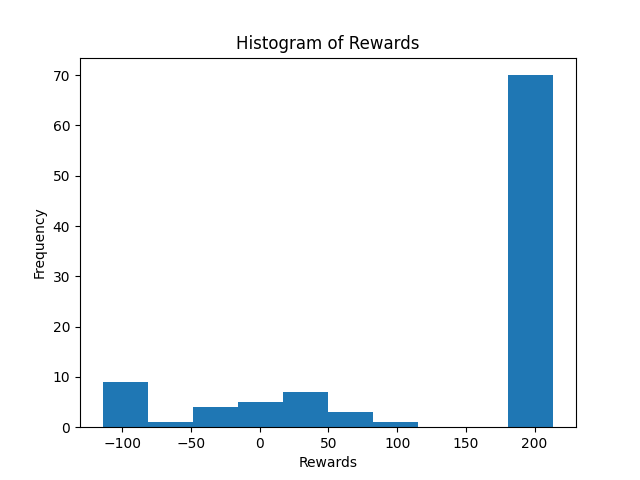
\includegraphics[width=0.4\textwidth]{histogramES.png}
			\caption{histogram of the rewards of the best agent}
			\label{fig:es_bipedalwalker}
		\end{figure}
		
		\subsection{PPO}
		In the PPO we used two networks, one for the policy and one for the value function. 




			
		
	\end{multicols}
	
	\begin{table}[H]
		\centering
		\begin{tabular}{cccc}
			\hline
			\celda{Nombres} & \celda{Apellidos} & \celda{Edad} & \celda{País}\\
			\hline
			\celda{Manuel} & \celda{Merino} & \celda{25} & \celda{Perú}\\
			\hline
			\celda{Pablo} & \celda{Perez} & \celda{27} & \celda{México}\\
			\hline
		\end{tabular}
		\caption{Esta es mi primera tabla en mi papaer}
		\label{tb: Tabla1}
	\end{table}

	\begin{multicols}{2}
		\lipsum[1]
		\section{Conociendo más de la Inteligencia Artificial.}
			\lipsum
		
		\lipsum[2]
		
		\section{Aplicación y Alcances}
			\lipsum
			
	    \begin{thebibliography}{00}
	    
	    \bibitem{Referencia1}
	        \newblock \textit{Título de la referencia 1}
	        \newblock Autor.
	        \newblock Año y editor.
	    
	    \bibitem{Referencia2}
	        \newblock \textit{Título de la referencia 2}
	        \newblock Autor.
	        \newblock Año y editor.
	        
	    \bibitem{Referencia3}
	        \newblock \textit{Título de la referencia 3}
	        \newblock Autor.
	        \newblock Año y editor.
	        
	    \bibitem{Referencia4}
	        \newblock \textit{Título de la referencia 4}
	        \newblock Autor.
	        \newblock Año y editor.
	    
	    \bibitem{Referencia5}
	        \newblock \textit{Título de la referencia 5}
	        \newblock Autor.
	        \newblock Año y editor.
	        
	    \bibitem{Referencia6}
	        \newblock \textit{Título de la referencia 6}
	        \newblock Autor.
	        \newblock Año y editor.
	    
	    \end{thebibliography}
	\end{multicols}
	
	\vspace{3cm}
	Para un mejor entendimiento de la plantilla ver el video en youtube:\\
	
	\url{https://www.youtube.com/watch?v=34xYuLxnzHo}
	
	
\end{document}